\subsection{Error State Kalman Filter}
While the Extended Kalman Filter provides a powerful framework for nonlinear estimation, it still linearizes directly around the full nominal state. For systems such as the Inertial Navigation System (INS), where the state includes both position, velocity, and attitude (represented by quaternions), this approach can lead to numerical inconsistencies, unstable orientation updates, and loss of orthogonality in rotation representations.  
\\ \\
To address these issues, the \textit{Error State Kalman Filter (ESKF)} reformulates the estimation problem by separating the system into two parts: a \textbf{nominal state} and a \textbf{small error state}. The nominal state follows the nonlinear dynamics of the INS, while the error state captures small deviations from this nominal trajectory. This approach allows the filter to maintain accurate nonlinear propagation of the nominal state while estimating only small, approximately linear error quantities.  
\\ \\
The nominal INS model is already defined earlier in this work as
$$
    \mathbf{x} =
    \begin{bmatrix}
        \mathbf{p} \\ \mathbf{v} \\ \mathbf{q} \\ \mathbf{b}_a \\ \mathbf{b}_g
    \end{bmatrix},
$$
where $\mathbf{p}$ is the position, $\mathbf{v}$ is the velocity, $\mathbf{q}$ is the attitude quaternion, and $\mathbf{b}_a$, $\mathbf{b}_g$ are the accelerometer and gyroscope biases. The nominal dynamics evolve as
$$
\begin{aligned}
    \dot{\mathbf{p}} &= \mathbf{v}, \\
    \dot{\mathbf{v}} &= \mathbf{R}(\mathbf{q})(\mathbf{a}_m - \mathbf{b}_a) + \mathbf{g}, \\
    \dot{\mathbf{q}} &= \tfrac{1}{2}\Omega(\boldsymbol{\omega}_m - \mathbf{b}_g)\mathbf{q}, \\
    \dot{\mathbf{b}}_a &= \mathbf{w}_{b_a}, \\
    \dot{\mathbf{b}}_g &= \mathbf{w}_{b_g},
\end{aligned}
$$
where $\mathbf{R}(\mathbf{q})$ is the rotation matrix from body to navigation frame, $\Omega(\cdot)$ is the quaternion multiplication matrix, $\mathbf{a}_m$ and $\boldsymbol{\omega}_m$ are the measured accelerations and angular rates, and $\mathbf{w}_{b_a}$ and $\mathbf{w}_{b_g}$ are random-walk noise processes on the biases.  
\\ \\
From this nominal model, the corresponding \textbf{error-state INS model} can be derived by linearizing around the nominal trajectory. Following Edmund Brekke’s formulation, the continuous-time error-state dynamics are expressed as
$$
    \dot{\delta\mathbf{x}} =
    \begin{bmatrix}
        \dot{\delta\mathbf{p}} \\ \dot{\delta\mathbf{v}} \\ \dot{\delta\boldsymbol{\theta}} \\ \dot{\delta\mathbf{b}}_a \\ \dot{\delta\mathbf{b}}_g
    \end{bmatrix}
    =
    A \, \delta\mathbf{x} + G\,\mathbf{w},
$$
where
$$
A =
\begin{bmatrix}
    \mathbf{0} & \mathbf{I} & \mathbf{0} & \mathbf{0} & \mathbf{0} \\
    \mathbf{0} & \mathbf{0} & -\mathbf{R}[\mathbf{a}_m - \mathbf{b}_a]_\times & -\mathbf{R} & \mathbf{0} \\
    \mathbf{0} & \mathbf{0} & -[\boldsymbol{\omega}_m - \mathbf{b}_g]_\times & \mathbf{0} & -\mathbf{I} \\
    \mathbf{0} & \mathbf{0} & \mathbf{0} & \mathbf{0} & \mathbf{0} \\
    \mathbf{0} & \mathbf{0} & \mathbf{0} & \mathbf{0} & \mathbf{0}
\end{bmatrix},
\qquad
G =
\begin{bmatrix}
    \mathbf{0} & \mathbf{0} & \mathbf{0} & \mathbf{0} \\
    \mathbf{R} & \mathbf{0} & \mathbf{0} & \mathbf{0} \\
    \mathbf{0} & \mathbf{I} & \mathbf{0} & \mathbf{0} \\
    \mathbf{0} & \mathbf{0} & \mathbf{I} & \mathbf{0} \\
    \mathbf{0} & \mathbf{0} & \mathbf{0} & \mathbf{I}
\end{bmatrix}.
$$
Here, $[\cdot]_\times$ denotes the skew-symmetric matrix corresponding to a vector cross product. The matrix $A$ describes how small perturbations in position, velocity, attitude, and bias evolve, while $G$ distributes process noise into the error dynamics.  
\\ \\
In the ESKF, the covariance matrix $P$ describes the uncertainty of the \textit{error state}, not the nominal state. The nominal state evolves through the nonlinear INS model, while the error state and its covariance evolve linearly using the matrices $A$ and $G$. This separation ensures well-behaved uncertainty propagation and prevents numerical instability caused by nonlinearities in the nominal equations.  
\\ \\
Discretization of the continuous error dynamics is critical for digital implementation. In theory, the discrete-time transition matrix is given by
$$
    F_d = e^{A\Delta t}, \qquad
    Q_d = \int_0^{\Delta t} e^{A\tau} G Q G^\top e^{A^\top\tau} d\tau.
$$
However, directly computing these expressions is infeasible in real-time embedded systems. Several discretization strategies exist:
\\ \\
The \textbf{Cayley–Hamilton series} offers an exact polynomial expansion of the matrix exponential using the characteristic polynomial of $A$. This method is mathematically elegant and useful for analytical algebraic studies, especially in time-varying systems where symbolic manipulation is desired. However, it is computationally expensive and not practical for onboard estimation due to the repeated evaluation of high-order polynomial terms.
\\ \\
The \textbf{Zero-Order Hold (ZOH)} method provides a more practical alternative. It assumes the control inputs and process noise remain constant within each sampling interval. The ZOH preserves the exact dynamics for linear time-invariant systems and ensures numerical stability. In practice, the ZOH discretization can be computed using the augmented matrix exponential:
$$
    e^{\begin{bmatrix} A & GQG^\top \\ 0 & 0 \end{bmatrix}\Delta t}
    =
    \begin{bmatrix}
        F_d & Q_d \\
        0 & I
    \end{bmatrix}.
$$
While theoretically sound, this method can still be expensive for real-time embedded systems.  
\\ \\
In this work, the \textbf{Padé approximation with scaling and squaring} is used to compute the matrix exponential efficiently. This method offers an excellent compromise between computational speed and numerical accuracy. It is robust even for large or ill-conditioned $A$ matrices and remains the preferred approach in practical navigation and sensor fusion systems. In general, one should avoid crude first-order approximations such as $F_d \approx I + A\Delta t$, as they may degrade filter consistency, cause covariance divergence, and lead to inaccurate state propagation under high-dynamic motion.  
\\ \\
The ESKF estimation process proceeds in several stages. During the \textit{prediction step}, the nominal state is propagated using the nonlinear INS equations, while the covariance is propagated using the linearized error model:
$$
\begin{aligned}
    \hat{\mathbf{x}}_{k|k-1} &= f(\hat{\mathbf{x}}_{k-1|k-1}, \mathbf{u}_{k-1}), \\
    P_{k|k-1} &= F_d P_{k-1|k-1} F_d^\top + Q_d.
\end{aligned}
$$
The \textit{update step} corrects the error state using the measurement model:
$$
\begin{aligned}
    K_k &= P_{k|k-1} H_k^\top (H_k P_{k|k-1} H_k^\top + R)^{-1}, \\
    \delta\hat{\mathbf{x}}_{k|k} &= K_k [\mathbf{z}_k - h(\hat{\mathbf{x}}_{k|k-1})], \\
    P_{k|k} &= (I - K_k H_k) P_{k|k-1}.
\end{aligned}
$$
The corrected error state $\delta\hat{\mathbf{x}}_{k|k}$ is then injected into the nominal state estimate:
$$
    \hat{\mathbf{x}}_{k|k} \leftarrow \hat{\mathbf{x}}_{k|k-1} \oplus \delta\hat{\mathbf{x}}_{k|k},
$$
where $\oplus$ denotes the nonlinear composition of nominal and error states (e.g., position addition, quaternion rotation update).  
\\ \\
After injection, the error state is reset to zero before the next iteration:
$$
    \delta\hat{\mathbf{x}}_{k|k} \leftarrow 0.
$$
For attitude states represented by quaternions, normalization is also performed after the correction step to maintain a valid unit quaternion:
$$
    \mathbf{q}_{k|k} \leftarrow \frac{\mathbf{q}_{k|k}}{\|\mathbf{q}_{k|k}\|}.
$$
This ensures the quaternion remains on the unit hypersphere, preserving a consistent rotation representation without magnitude drift.  
\\ \\
Overall, the ESKF achieves greater numerical stability, robustness, and consistency than the EKF by estimating only small, well-behaved error quantities. The separation between the nonlinear nominal state and linear error state provides a strong balance between accuracy and computational efficiency. Consequently, the ESKF has become the standard approach for inertial navigation and sensor fusion applications involving rotational dynamics.
\\ \\
\begin{figure}[H]
    \centering
    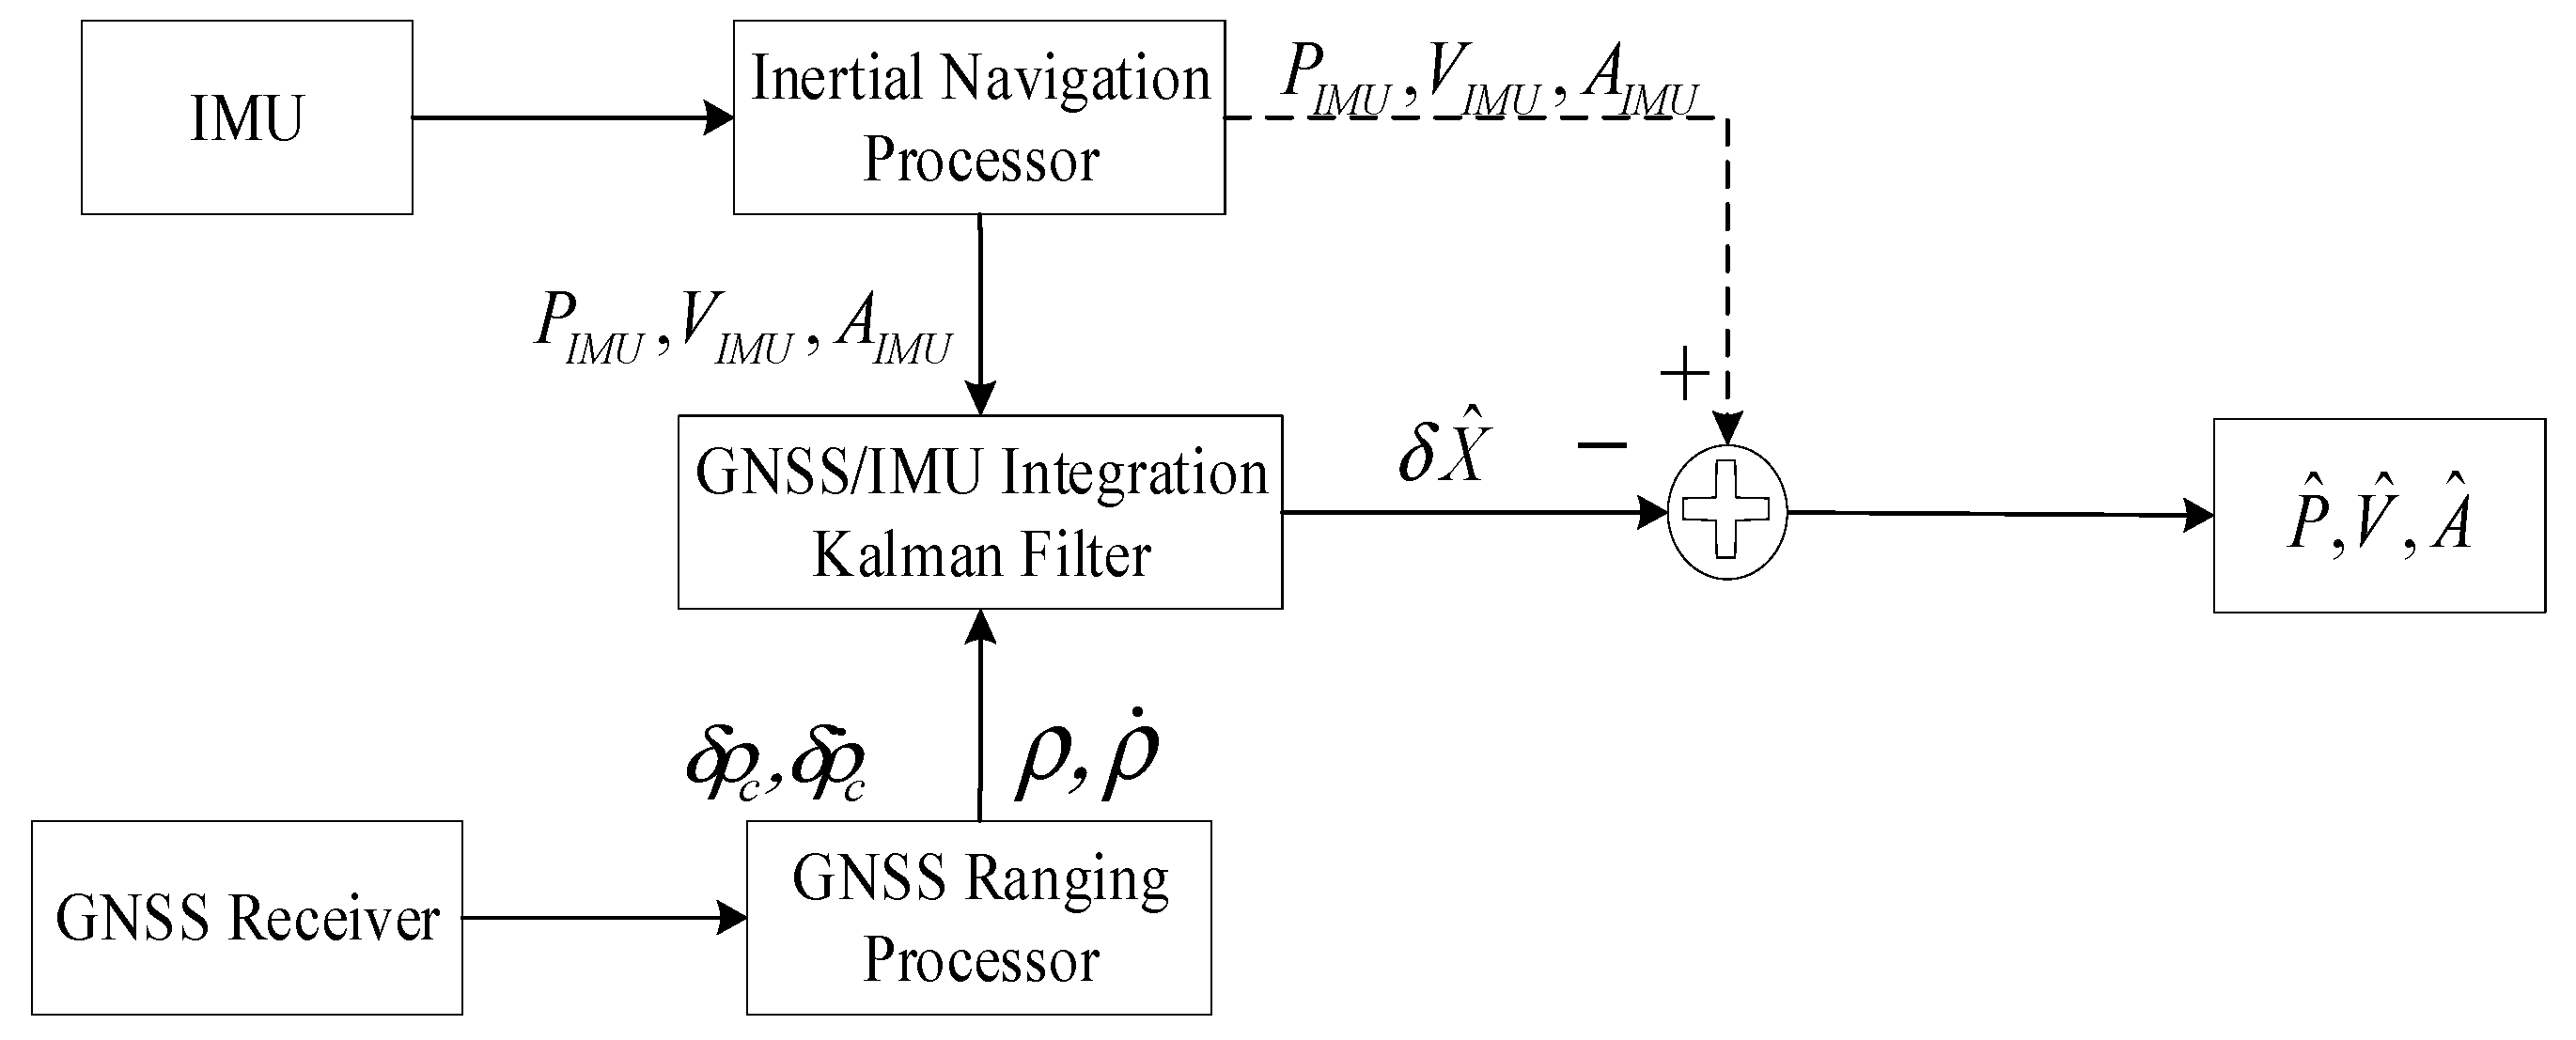
\includegraphics[width=1.0\linewidth]{Pictures/State_Estimation/Error_State_Kalman_Filter/Error_State_Kalman_Filter_Illustrated.png}
    \caption{Functional overview of the ESKF architecture. The Inertial Navigation System (INS) propagates the \textit{nominal states} --- position, velocity, and attitude --- based on IMU measurements. The GNSS receiver provides external position and velocity updates, which are processed through the GNSS ranging processor to generate pseudorange and pseudorange-rate measurements. The GNSS/IMU integration Kalman filter estimates the small \textit{error states} $\delta\hat{\mathbf{X}}$ between the predicted INS trajectory and the measured GNSS solution. These estimated errors are then re-injected into the nominal INS states to correct them, after which the error states are reset to zero. This closed-loop structure ensures stable and consistent state estimation by combining high-rate IMU propagation with low-rate GNSS corrections. Image adapted from a paper on the Error State Kalman Filter.\textsuperscript{\cite{error_state_kalman_filter}}}
    \label{fig:state-estimation-error-state-kalman-filter}
\end{figure}

